\documentclass{article}
\usepackage{graphicx}
\usepackage{subcaption}


\begin{document}
	\section{Motivation}
	The programming language is python. The basic algorithm is the nearest centroid mean algorithm. The algorithm initially compute the mean for each class. The mean is a vector which is computed by averaging two features of training data. The algorithm to classify data is to compute the Euclidean distance between feature vector and  mean vector trained by the classifier. 	 
	\section{Problem solution}
	\subsection{problem a}
	Two figures are generated by using \textit{PlotDecBoundaries()}. The CSV file is read by the library supported by the numpy. The data is stored into the \textit{ndarray}.  The Figure \ref{fig:synthetictrain1} shows the data points, class mean and decision boundary for synthetic data set 1. The Figure \ref{fig:synthetictrain2} shows these information for synthetic data set 2. 
	\begin{figure}[hbt!]
		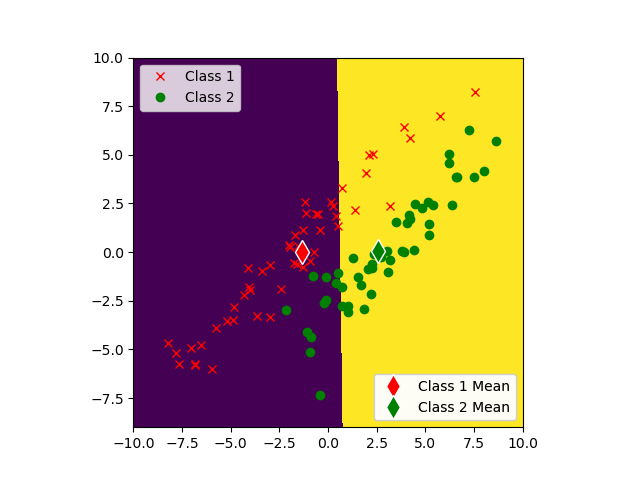
\includegraphics[width=\linewidth]{images/synthetic_trian1.png}	
		\caption{synthetic train1}
		\label{fig:synthetictrain1}
	\end{figure}
	\begin{figure}[hbt!]
		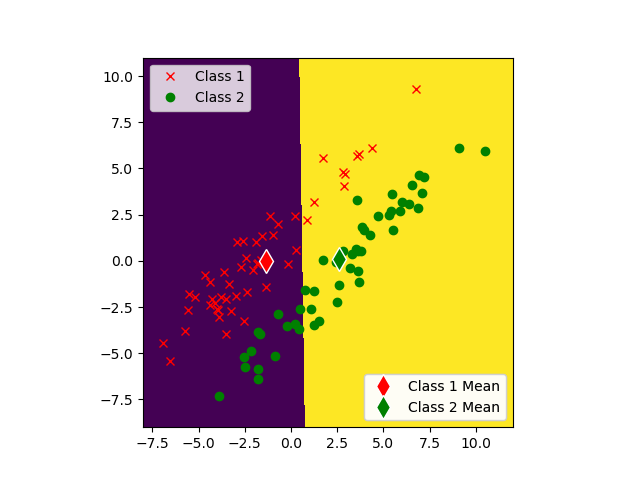
\includegraphics[width=\linewidth]{images/synthetic_test1.png}
		\caption{synthetic test1}
		\label{fig:synthetictest1}
	\end{figure}
	\begin{figure}[hbt!]
		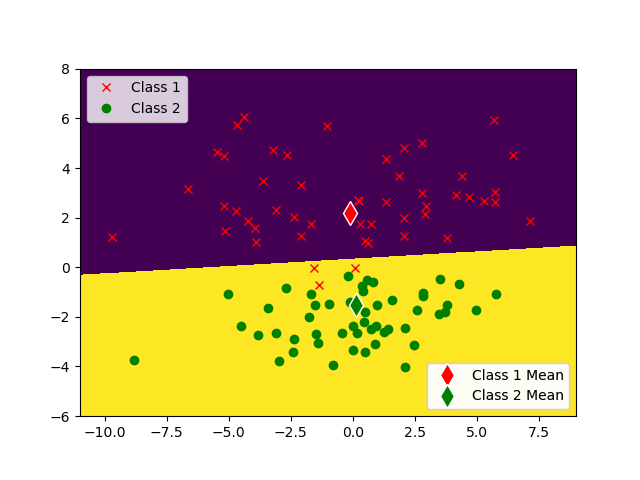
\includegraphics[width=\linewidth]{images/synthetic_train2.png}
		\caption{synthetic train2}
		\label{fig:synthetictrain2}
	\end{figure}
	\begin{figure}[hbt!]
		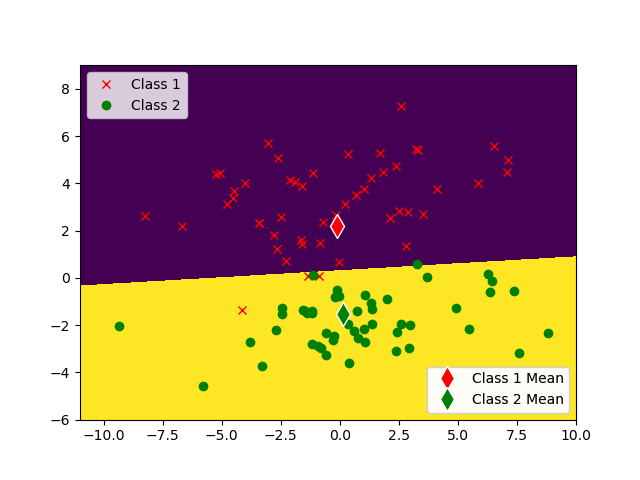
\includegraphics[width=\linewidth]{images/synthetic_test2.png}
		\caption{synthetic test2}
		\label{fig:synthetictest2}
	\end{figure}
		\begin{table}[hbt!]
		\begin{center}
		\begin{tabular}{| l | l | l | p{5cm} |}
		\hline
			Data      & Error rate & Test samples  \\ \hline
			synthetictrain1& 0.24        & 100    \\  \hline
			synthetictest1& 0.24		& 100    \\   \hline
			synthetictrain2& 0.04        & 100    \\  \hline
			synthetictest2& 0.04		& 100    \\   \hline
		\end{tabular}
		\end{center}
	\caption{Error rate}
	\label{table: errorrate}
	\end{table}
	 \\
	\subsection{problem b}
	The error rate of both synthetic data set is shown in the table \ref{table: errorrate}. The table also shows the error rate of the synthetic data set 2 is smaller than the error rate of the synthetic data set 1. The performance of data set 2 is also good in the training data set. The class error is computed by running python program synthetic.py. The console display the error rate. The error rate for both data set 1 and 2 is the same when the error rate of training  data and error rate of testing data is compared. If the error rate is different for test set and train set, this means some data is not collected for some reason. The train set is not complete and can not fully represent the class. As error rate in our data set is the same, there is no problem for data collection of training data set. If error rate is very high, this means the algorithm perform bad for classification.    
	\subsection{problem c}
		\begin{figure}[hbt!]
		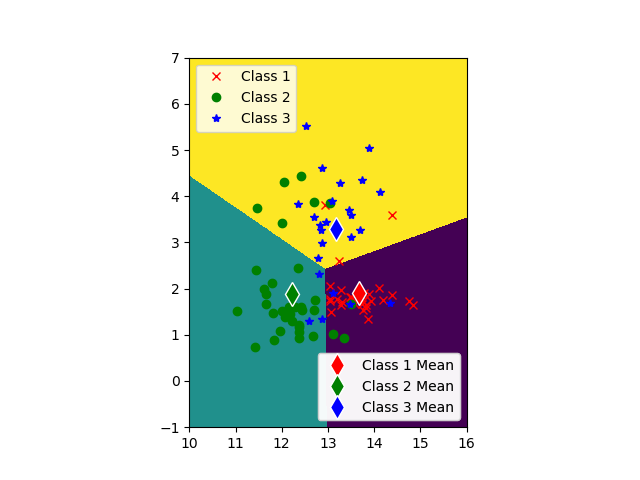
\includegraphics[width=\linewidth]{images/wine_feature01_train.png}	
		\caption{the data scatter plot of wine data set whose feature is 0 and 1}
		\label{fig:wine_feature01_train}
		\end{figure} 
	The Figure \ref{fig:wine_feature01_train} shows the training data points, sample mean and decision boundary for wine data set. The sample mean is produced by the feature 1 and 2 of training data. Error rate of the train data was shown in the table \ref{table: wineerrorrate}.                                
	\subsection{problem d}
		\begin{table}[hbt!]
		\begin{center}
			\begin{tabular}{| l | l | l  | p{5cm} |}
				\hline
				Description     & Error rate(Train Data) & Sample Number    \\ \hline
best feature 1 and 12 (train data)     &0.079    &    89    \\      \hline
feature 1 and 2 (train data)  & 0.020	  &	   89     \\      \hline
best feature 1 and 12 (test data)	   & 0.742     &    89       \\      \hline
feature 1 and 2 (test data)      & 0.224	  &	   89      \\      \hline
feature 2 and 3 (train data)	   & 0.393    &    89       \\      \hline
feature 2 and 3 (test data)      & 0.730	  &	   89      \\      \hline
feature 2 and 4 (train data)	   & 0.393    &    89       \\      \hline
feature 2 and 4 (test data)      & 0.674	  &	   89      \\      \hline
			\end{tabular}
		\end{center}
		\caption{Error Rate for wine data set}
		\label{table: wineerrorrate}
	\end{table}
	\begin{figure}[hbt!]
		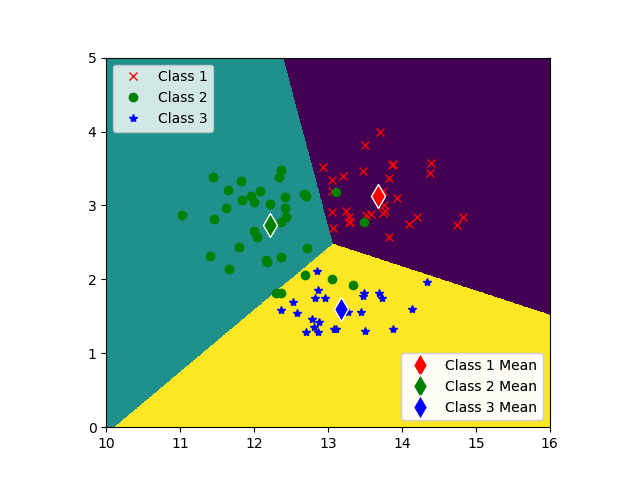
\includegraphics[width=\linewidth]{images/best_features_wine.png}	
		\caption{graph produced by the feature 1 and 12 of train data}
		\label{fig: bestFeature}
	\end{figure} 
	The Figure \ref{fig: bestFeature} has shown boundaries of best features. The principle to select best feature is to compare the error rate of the training data. The feature which produces the lowest error rate is selected. All combination of two features in thirteen feature was compared. The best features were selected to produce the Figure \ref{fig: bestFeature}. The table \ref{table: wineerrorrate} also provided some error rates of different pair of features. 
	\subsection{problem e}
	The mean of error rate of all pairs of two selected feature of train data is 0.336, and the variance of error rate is 1.285.  The result was generated by program $wine.py$ . The error rate for test data is much higher than the error rate of train data. 
	From comparison between error rate of train data and test data of chosen best pair of features, the best features seem to be over fitting for the train data set because the error rate of test data set is extremely high for the same selected feature. The correlation between test data error rate and train data error rate is small. Hence, the selected best features  can not perfectly classify the test data. The possible problem may be the deficiency of features numbers. 
	\section{Summary}
	The nearest centroid mean algorithm performs well on synthetic data set. For real problem of wine classification, some features have small error rate for train data. The error rate of test data of same features is high. This case presents the defect of the algorithm. The selected features are over-fitting for train data set. 
\end{document}